\documentclass[12pt]{article}
\usepackage[latin1]{inputenc}
\usepackage[english]{babel}
\usepackage{amsmath}
\usepackage{amssymb}
%\usepackage{dsfont}
\usepackage{theorem}
\usepackage{graphicx}
\usepackage{hyperref}
\usepackage{lscape}
\usepackage{enumerate}
\usepackage{verbatim}
\usepackage{float}
\usepackage{fancyhdr}
%\usepackage{bigints}
\pagestyle{fancy}




\newcommand{\dif}{\mbox{d}}


%---------------------------------
%\topmargin -.5 in
%\textheight 22 cm
%\textwidth 16 cm
%\oddsidemargin 0 cm
%\evensidemargin 0 cm
%---------------------------------


\title{Growing Degree Days in Canada - Data Project}
\author{A. Naveen, C. Chagas, A. Iyer, O. Abramov, E. Kielley, R. Brecht}
\date{\today}

\begin{document}

\maketitle
\vspace{20pt}%\vspace{5pt}
\tableofcontents
%\vspace{35pt}
\pagebreak
\section{Motivation}
We want to use Python and Bash scripts to analyse growing degree days (GDD) for 
three different cities in Canada. Growing degree days are used to predict when a 
flower or plant will bloom. 
\\ Plants require energy to grow and develop, and some of this energy is in the 
form of heat. The heat required is expressed as degrees of temperature. 
Temperature regulates many of the physical and chemical processes within a 
plant, which in turn control the rate of growth and development toward maturity. 
\\The amount of heat accumulated during the day, as obtained by subtracting the
 plant's base temperature from the mean temperature for the day, is termed the
 degree-day accumulation.
\\The growing degree days helps to identify the limits of geographical areas 
suitable for production of various crops, particularly corn, and to evaluate 
areas agriculturally suitable for new or non-native plants. Other applications
of degree-days include the prediction of bloom date, tree fruit development, and
insect activity related to agriculture and forestry.
\\The aim of this project was to gain experience in computational workflow for a
scientific problem involving GDD calculations and plots creation. The three cities 
chosen to develop the minimum tasks were Montreal, Victoria and Ottawa.


\pagebreak

\section{Program Structure}
\subsection{Files and Scripts}
\begin{description}
\item[gdd.py]
\item Input: tbase, tupper, input\_folder (optional)
\item Output: year\_cityName\_tbase\_tupper\_gdd.csv
\item Searches for files that ends with \emph{temp.csv}. These
files should have the columns: Date/Time, Min Temp(${}^\circ$C), Max Temp(${}^\circ$C).
The csv files can be found at \cite{CityTemp}.

Then the columns of each file will be copied into a new csv file with the name
\emph{year\_cityName\_tbase\_tupper\_gdd.csv}, where cityName is extracted from the
current file name. That file will be saved in the folder \emph{Output}.
In this file, a new column called GDD will be added. The GDD values of that column 
will be calculated by calling \emph{calc\_gdd.py}.
Then the value of cell $n$ is calculated with the formula:
$$
\sum_{i=1}^n \big( \tfrac{\text{tmax}_i+\text{tmin}_i}{2}-\text{tbase}\big)
$$
If $\text{tmax}_i$ or $\text{tmax}_i$ is bigger than tupper it is set to tupper,
 also if $\text{tmin}_i$ or $\text{tmax}_i$ 
is  smaller than tbase then it is set to tbase.
\\The base temperature, Tbase, is that temperature below which plant growth is zero.
 Growing Degree Units (GDUs) are accumulated by adding each day's GDs contribution as the season progresses.
\\ The maximum temperature, Tupp, is usually capped at 30 ${}^\circ$C because most plants and 
insects do not grow any faster above that temperature.
%\item[gdd.sh]
%\item Input: temperatures.csv, tbase, tupper
%\item Output:
%\item What it does... maybe adding code

\item[bokeh\_serve\_gdd.py]
\item Can be called by the comand line with \emph{$--$ show bokeh\_serve\_gdd.py} .
Shows the cumulative GDD for the 14 capital cities in Canada (Task 2.5).

\item[create\_plots.py]
\item Output: CumulativeGDD.png, CompareMaxMinTemp.png, AnalyzeTbase.png, gddMapPlotNL.png
\item The script consists of functions:

\begin{itemize}
\item max\_min\_plot(names) $\to$ CompareMaxMinTemp.png \\
Shows the maximum and minimum temperatures for Monteral, Ottawa and Victoria during the year of 2015 (Task 1.2).

\item gdd\_plot(names)  $\to$ CumulativeGDD.png \\
Shows the cumulative GDD for Montreal, Ottawa and Victoria in the year of 2015 (Task 1.4).

\item bokeh\_plot\_gdd\_years() $\to$ OptionalTask1GDDPlot.html \\
Shows the GDD stats for Ottawa. 

\item map\_plot\_nl\_gdd()  $\to$  gddMapPlotNL.png \\
Creates a colored map showing how the growing degree days accumulation affects Newfoundland (Task 2.2).

\item analyze\_tbase()  $\to$ Analyze\_Tbase.png \\
Shows the accumulated GDD in Victoria when the tbase is different from the default (Task 2.3).

\item bokeh\_plot\_temp(fname) $\to$ base\_temp.html \\
Shows interactively the minimum and maximum temperatures for Victoria in 2015 (Task 2.4.1).

\item bokeh\_plot\_gdd(fname) $\to$ base\_gdd.html \\
Shows the interactive plots in html format for Victoria in 2015 (Task 2.4.2).

\item plot\_lin\_reg(city,startYear, endYear,tbase,tupper) $\to$ LinReg\_Toronto\_1960\_2015.png \\
Shows the accumulated GDD for Toronto from 1960 to 2015.

\item make\_map\_plots() $\to$ gddMapPlotNL.png, CanadaBloomingOfMaple.png \\
Shows the blooming month of maple trees in Canada (Final Task).
Reads the csv files \emph{tempMin.csv, tempMax.csv, canadaMean.csv}, which can 
be downloaded from \cite{gridTemp}, into pandas dataframe and extracts latitude, 
longitude and calculates the gdd or blooming month for each grid point 
(which is also stored in a variable called gdd).
Then calls the function \emph{map\_plot(lat, lon, gdd,...)}. That function
interpolates the given gdd for a finer grid on the map. Then creates a map plot
showing just the interpolated data.
\end{itemize} 


\end{description}
\subsection{Process flow}
The following diagramm shows the dependencies and execution steps of the scripts
we are running.
\\~\\
By executing the \emph{Makefile}, we create a folder called \emph{Output} and run
the python script \emph{gdd.py} with the arguments tbase=10, tupper=30 and the path
 \emph{./Input/}. This produces 3 csv files, because we have 3 files of the 
format \emph{year\_cityName\_.csv} in the folder \emph{Input}.
Next the script \emph{create\_plots.py} is called by Makefile and produces  PNG- and html
files. Finally Makefile creates the file \emph{report.pdf} by compiling the 
\emph{report.tex} file.

	\begin{figure}[!htbp]
		\centering
		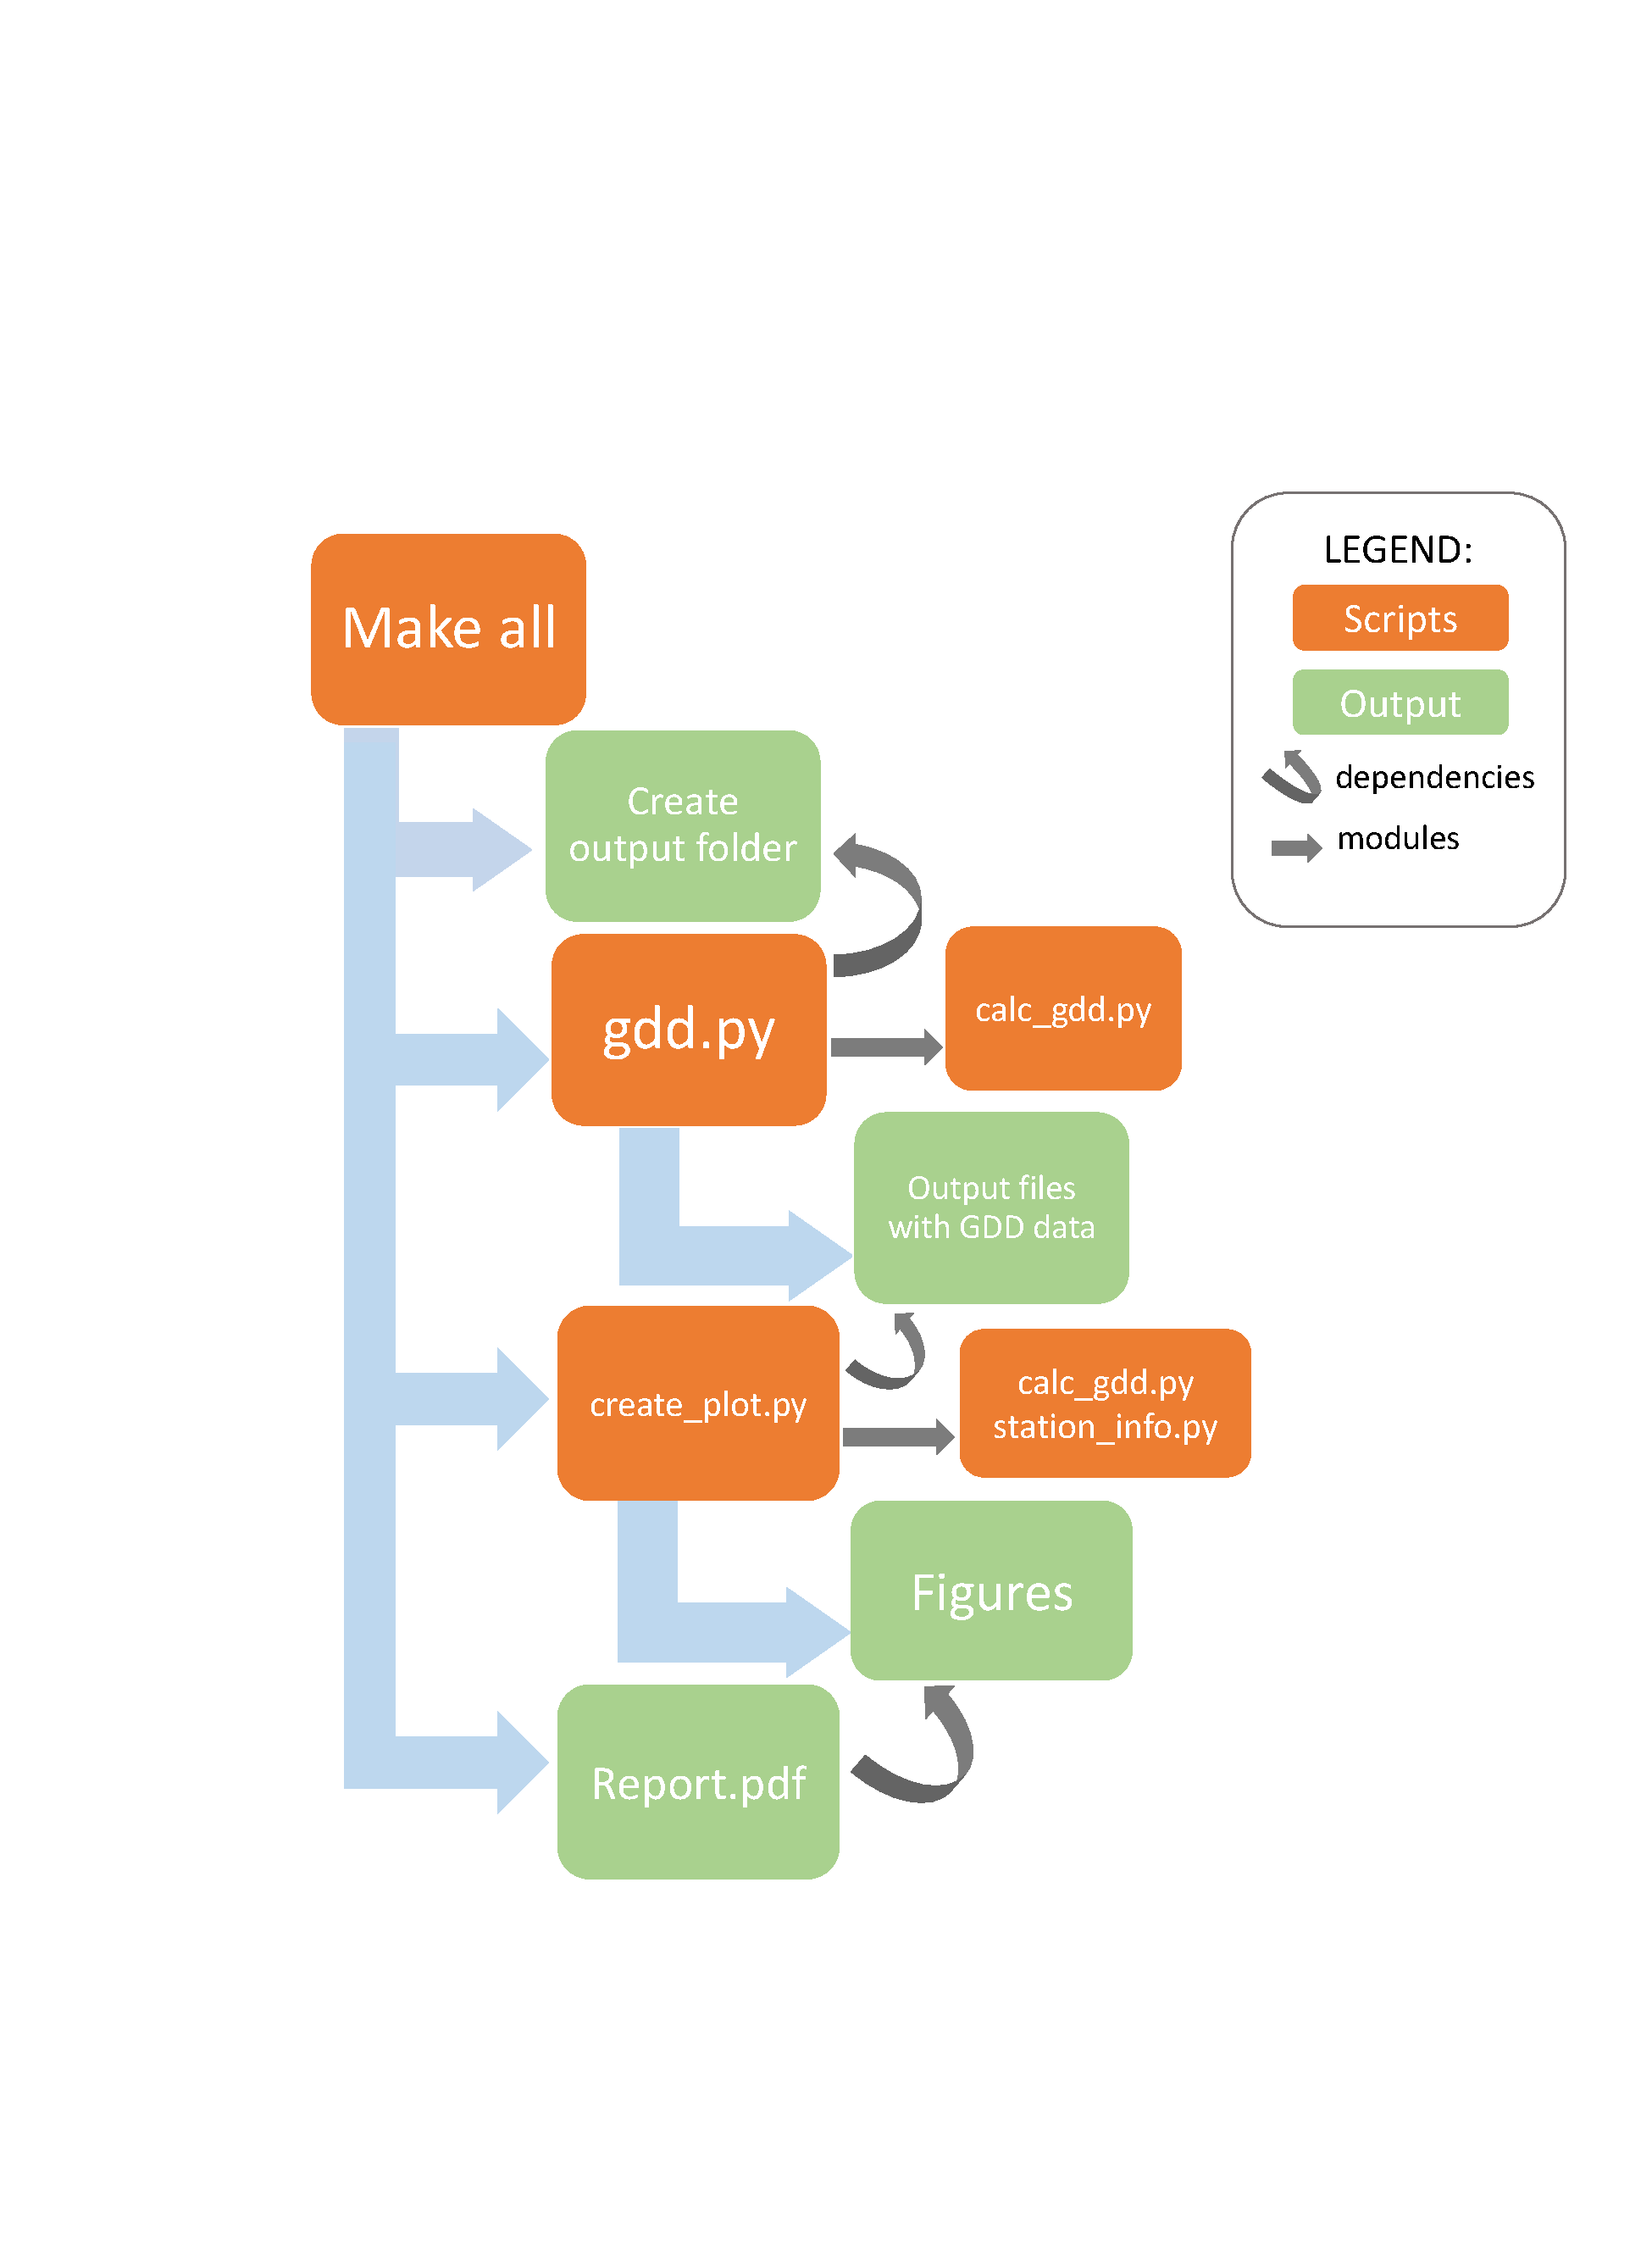
\includegraphics[width=0.9\textwidth]{./Report/diagram_workflow.pdf} 
		\caption{\scriptsize Shows the process flow of our scripts.}\label{flowplot}		  
	\end{figure}


\pagebreak
\section{Results}
Below are the the plots for the different tasks. 
The following table shows which figure belongs to which task:
\begin{center}
\begin{tabular}{l l}
Figure & Task\\
\hline
Figure \ref{MinMaxplot} & Task 1.2\\
Figure \ref{GDDplot}    & Task 1.4\\
Figure \ref{GDDstats}  & Task 2.1\\
Figure \ref{gddMapNl} & Task 2.2\\
Figure \ref{analyzeTbase} & Task 2.3\\
Figure \ref{bokehTempMontreal} & Task 2.4\\
Figure \ref{bokehAccGDD} & Task 2.4\\
Figure \ref{BokehServer} & Task 2.5\\
Figure \ref{LinReg} & Task 2.6\\
Figure \ref{gddMapCaMaple} & Final Task
\end{tabular}
\end{center}

	\begin{figure}[!htbp]
		\centering
		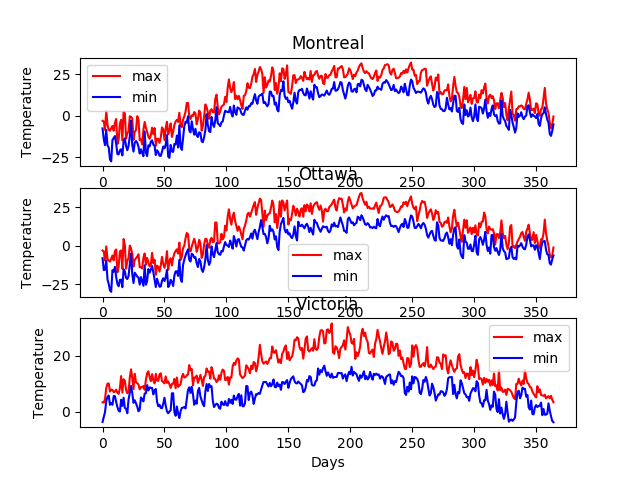
\includegraphics[width=0.9\textwidth]{./Output/CompareMaxMinTemp.png} 
		\caption{\scriptsize Shows the min and max temperatures for Montreal, Ottawa and Victoria 
		where it can be seen that both Montreal and Ottawa had lower and higher temperatures than 
		Victoria in 2015.}\label{MinMaxplot}		  
	\end{figure}


	\begin{figure}[!htbp]
		\centering
		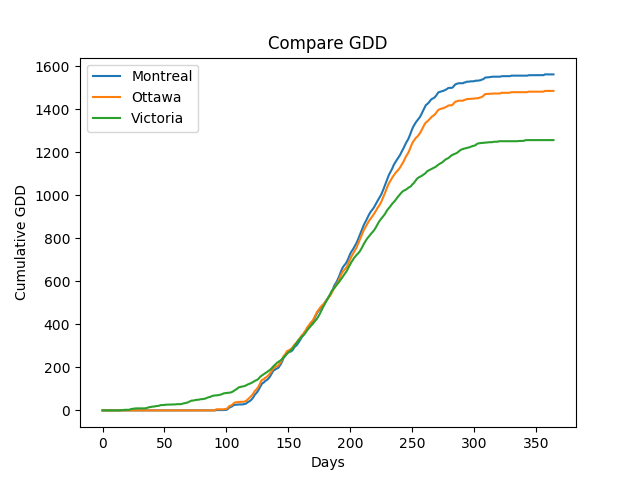
\includegraphics[width=0.9\textwidth]{./Output/CumulativeGDD.png} 
		\caption{\scriptsize Shows the accumulated GDD vs time for Montreal, Ottawa and Victoria also
		during 2015.}\label{GDDplot}		  
	\end{figure}

	\begin{figure}[!htbp]
		\centering
		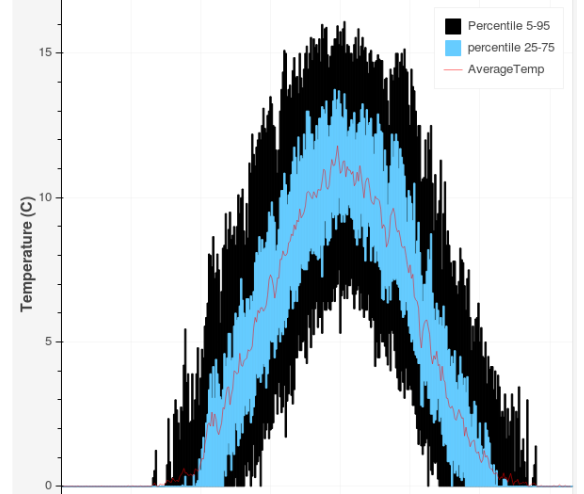
\includegraphics[width=0.9\textwidth]{./Report/GDDstats.png} 
		\caption{\scriptsize Shows the average GDD for Ottawa from 1960 to 2016.}\label{GDDstats}		  
	\end{figure}


	\begin{figure}[!htbp]
		\centering
		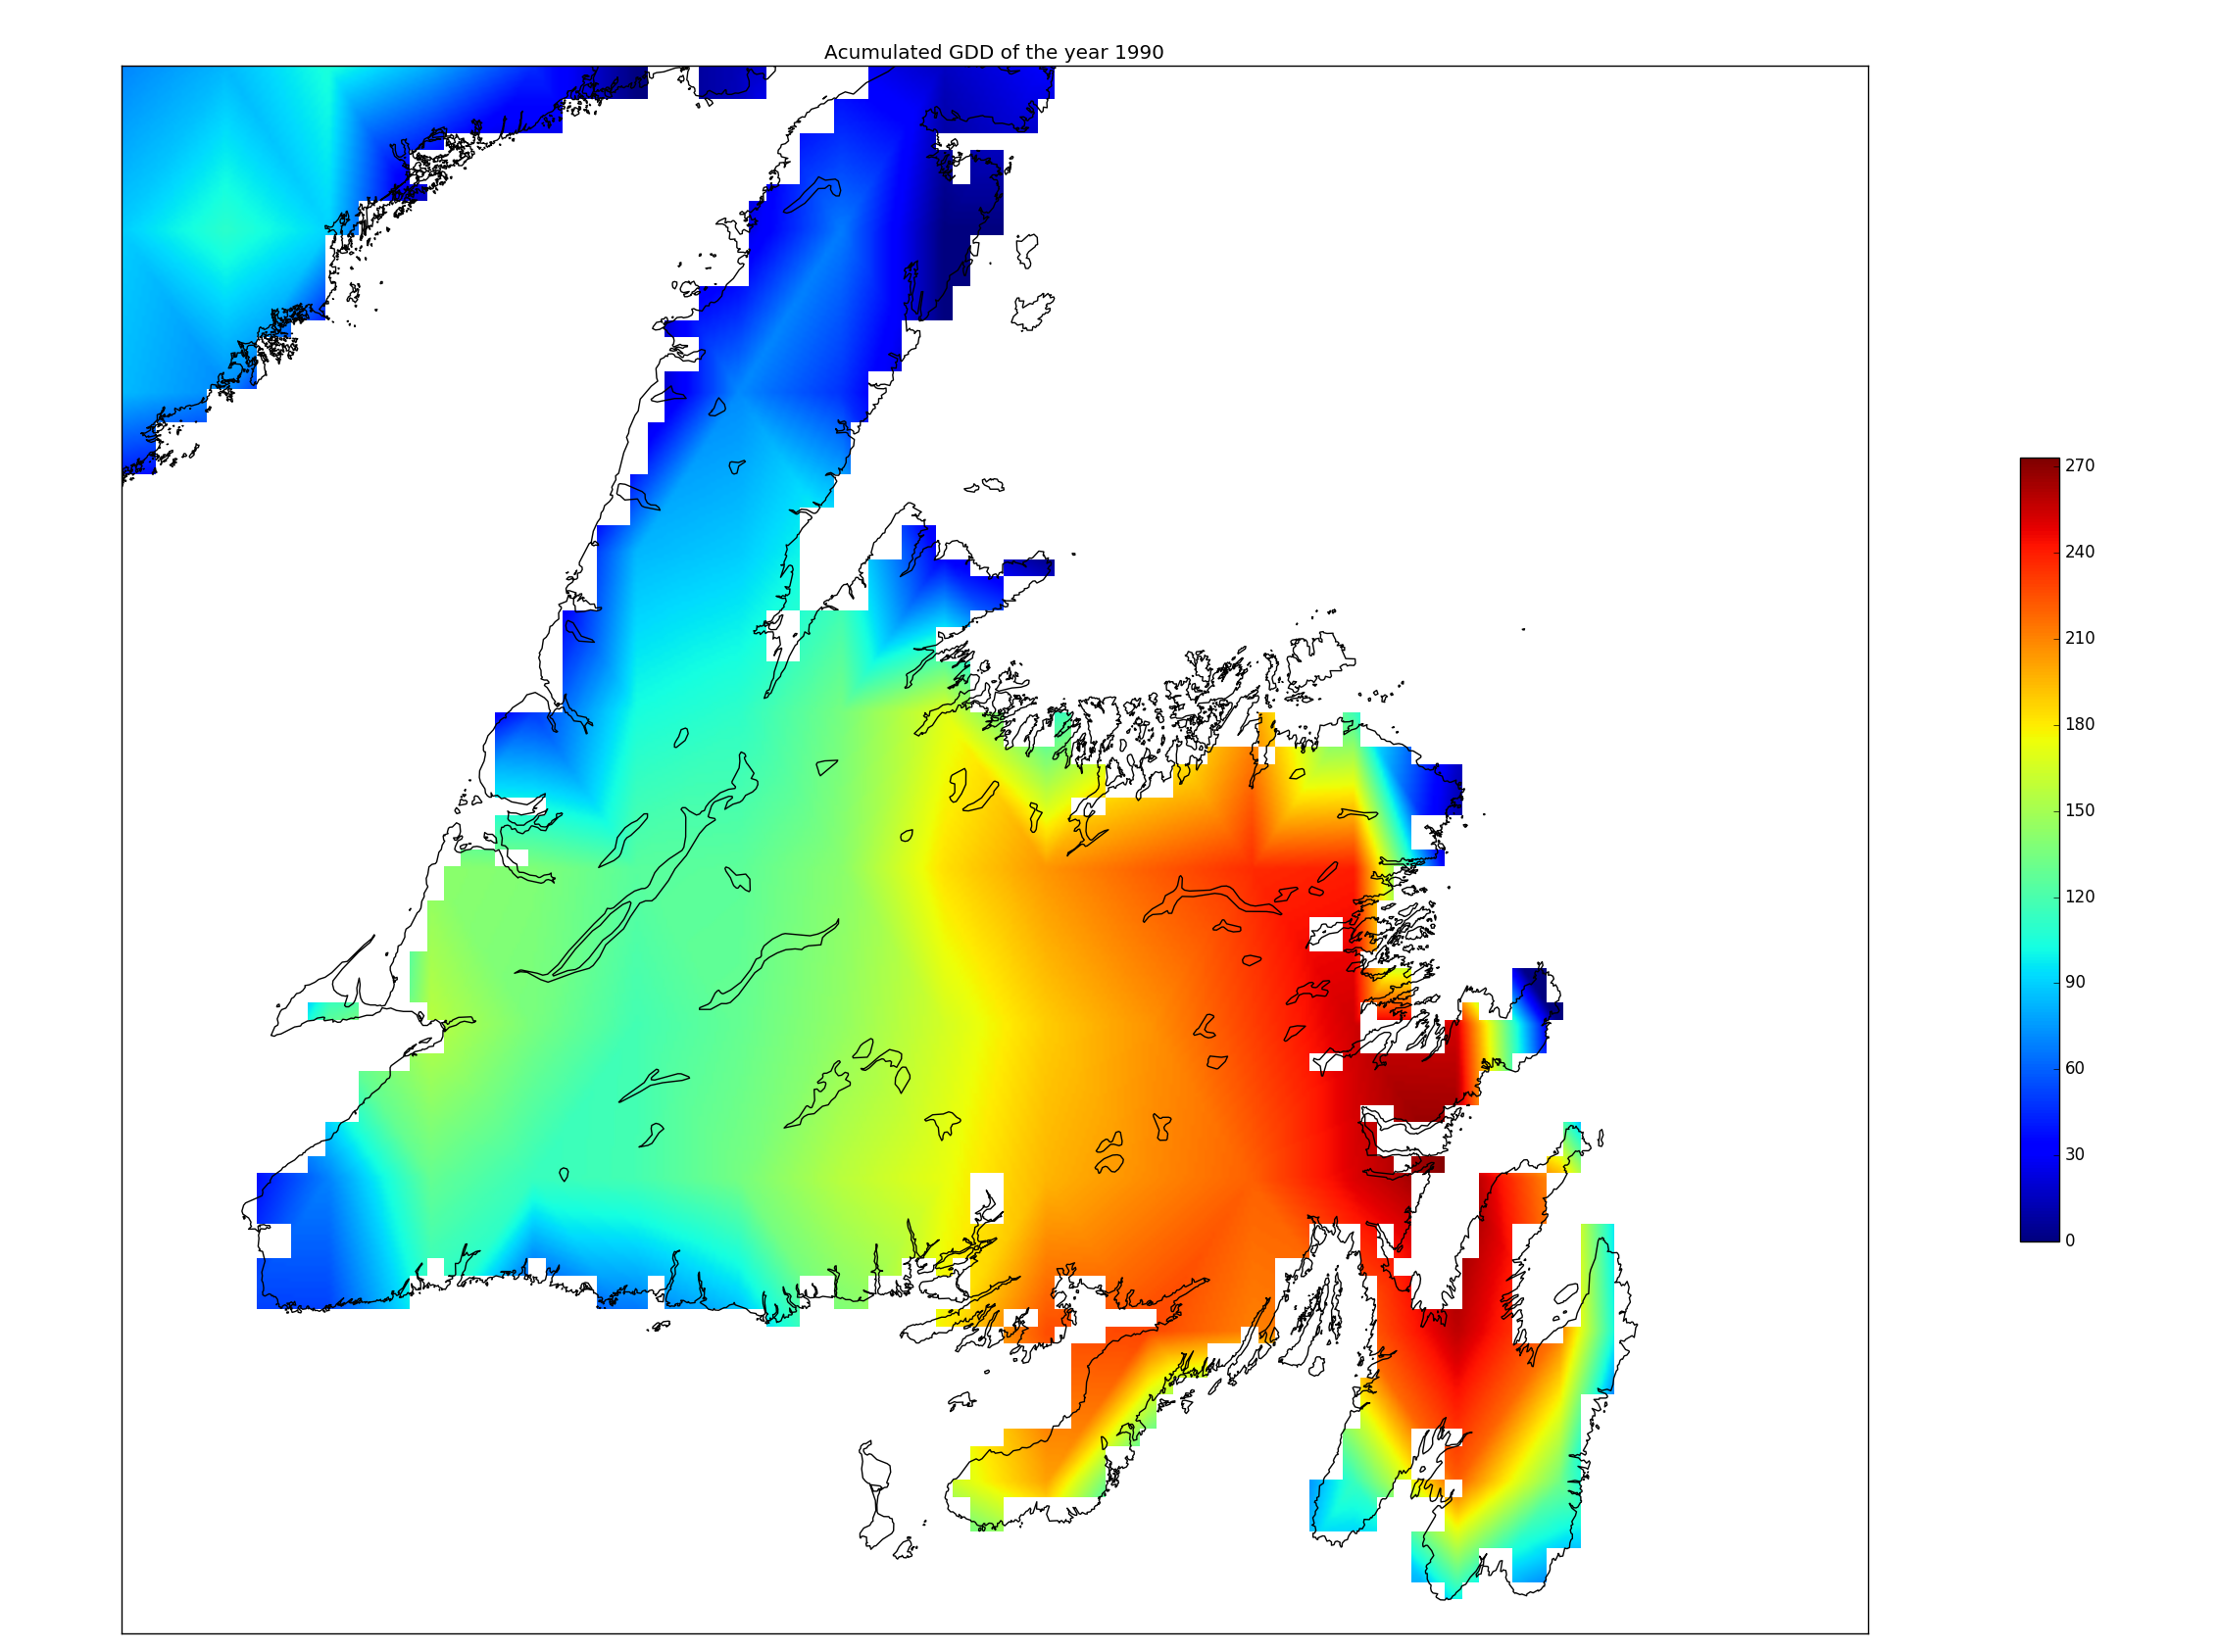
\includegraphics[width=0.9\textwidth]{./Output/gddMapPlotNL.png} 
		\caption{\scriptsize Shows the growing degree days accumulation of Newfoundland, 
		in which can be seen that the costal areas of the island are in colder colors when compared to
		inland probably due to the effect caused by the ocean air.
		}\label{gddMapNl}		  
	\end{figure}

	\begin{figure}[!htbp]
		\centering
		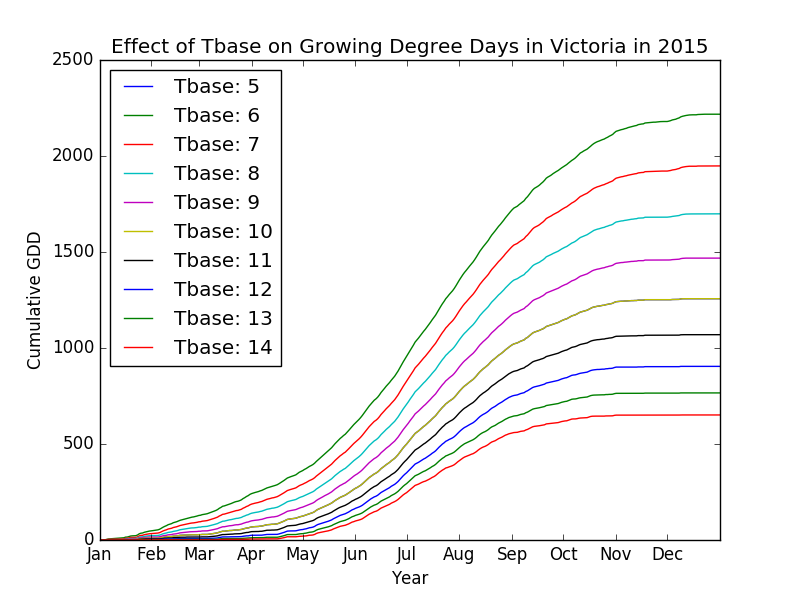
\includegraphics[width=0.9\textwidth]{./Output/AnalyzeTbase.png} 
		\caption{\scriptsize The plot shows how GDD is affected when changing the Tbase. If
		Tbase is increased by 11 for example, less accumulation of GDD is seen along the days. As Tbase 
		decreases, more temperature is accumulated. Data is shown for Victoria in 2015..}\label{analyzeTbase}		  
	\end{figure}

	\begin{figure}[!htbp]
		\centering
		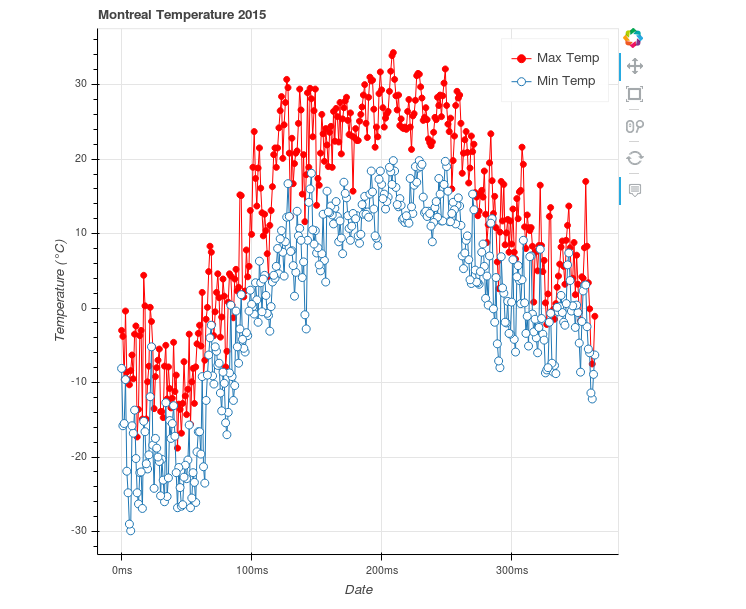
\includegraphics[width=0.9\textwidth]{./Report/tempMontreal.png} 
		\caption{\scriptsize Interactive bokeh plot for minimun and max temperatures of
		Victoria in 2015.}\label{bokehTempMontreal}		  
	\end{figure}
	
	\begin{figure}[!htbp]
		\centering
		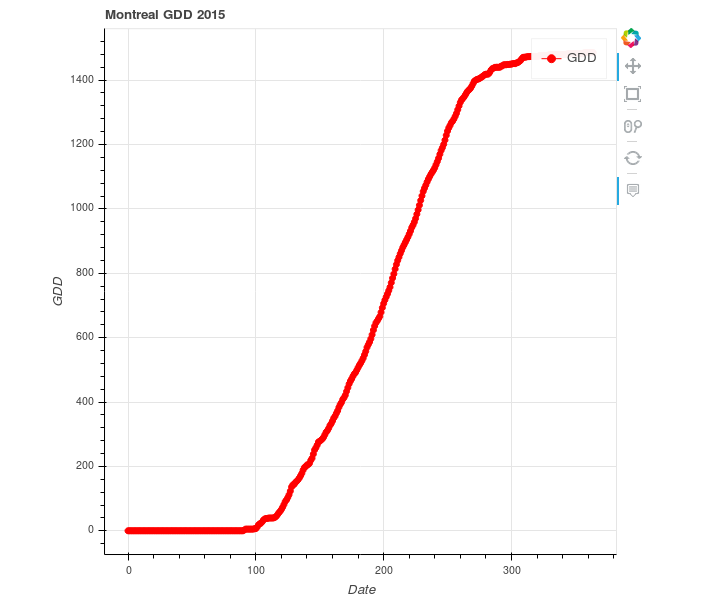
\includegraphics[width=0.9\textwidth]{./Report/accGDD.png} 
		\caption{\scriptsize Bokeh plot for accumulated GDD in Victoria in 2015.}\label{bokehAccGDD}		  
	\end{figure}
	
	\begin{figure}[!htbp]
		\centering
		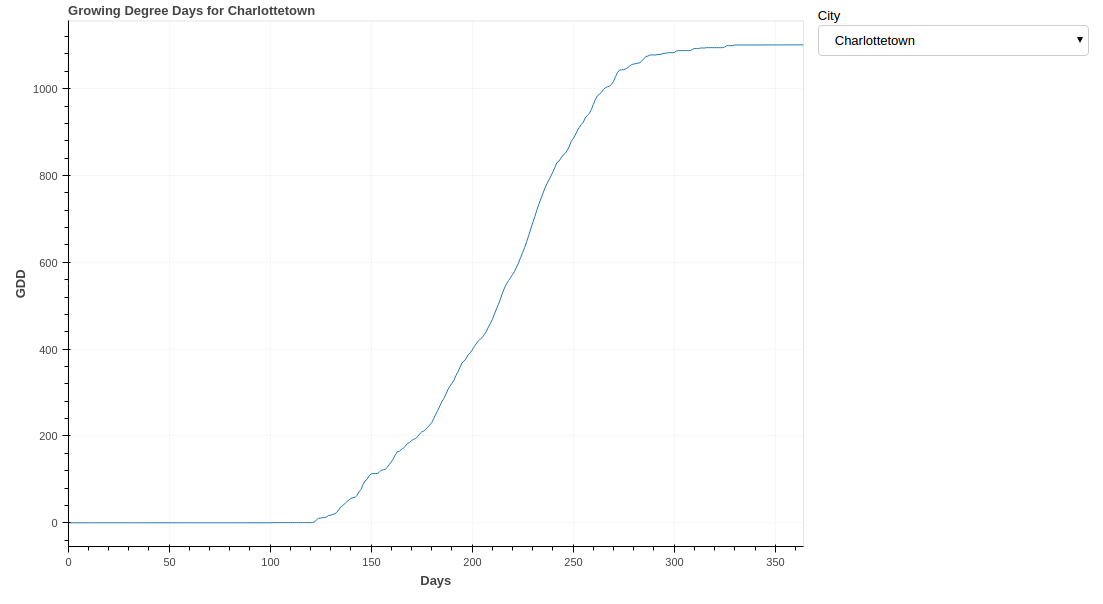
\includegraphics[width=0.9\textwidth]{./Report/bokeh_serve_screenshot.png} 
		\caption{\scriptsize Figure shows a screenshot of the online bokeh server plot showing the
		GDD for Charlottetown in 2015.}\label{BokehServer}		  
	\end{figure}
	
	\begin{figure}[!htbp]
		\centering
		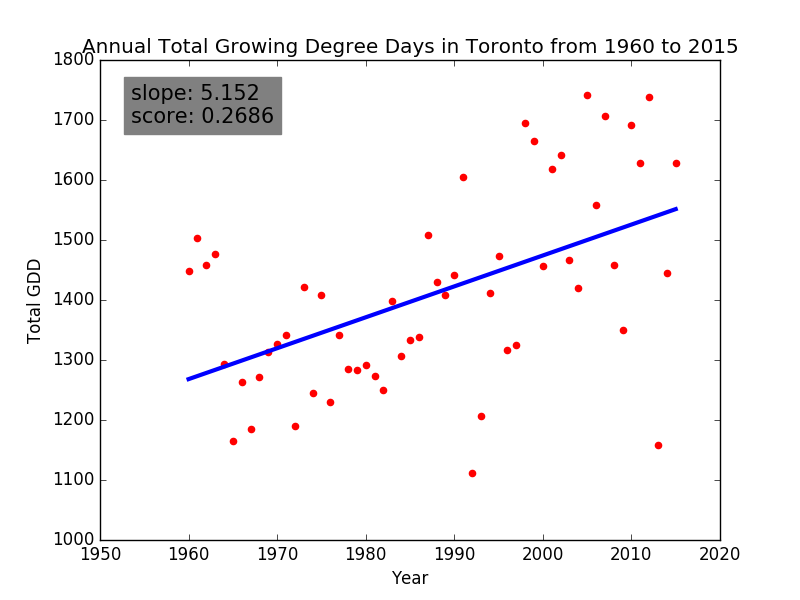
\includegraphics[width=0.9\textwidth]{./Output/LinReg_Toronto_1960_2015.png} 
		\caption{\scriptsize Figure shows the linear regression for Toronto from 1960 to 2015, 
		in which the total GDD around 1965 for example, was 1200, but in 2015 it was close to 
		1600 showing how the climate change is warming and affecting the planet.}\label{LinReg}		  
	\end{figure}

%For example, suppose you plant Red Maple in different areas on May 15th.
%The tree has a base temperature of 10${}^\circ$C and requires 27 GDD to reach maturity.
%See figrue \ref{gddMapCaMaple}.
	\begin{figure}[!htbp]
		\centering
		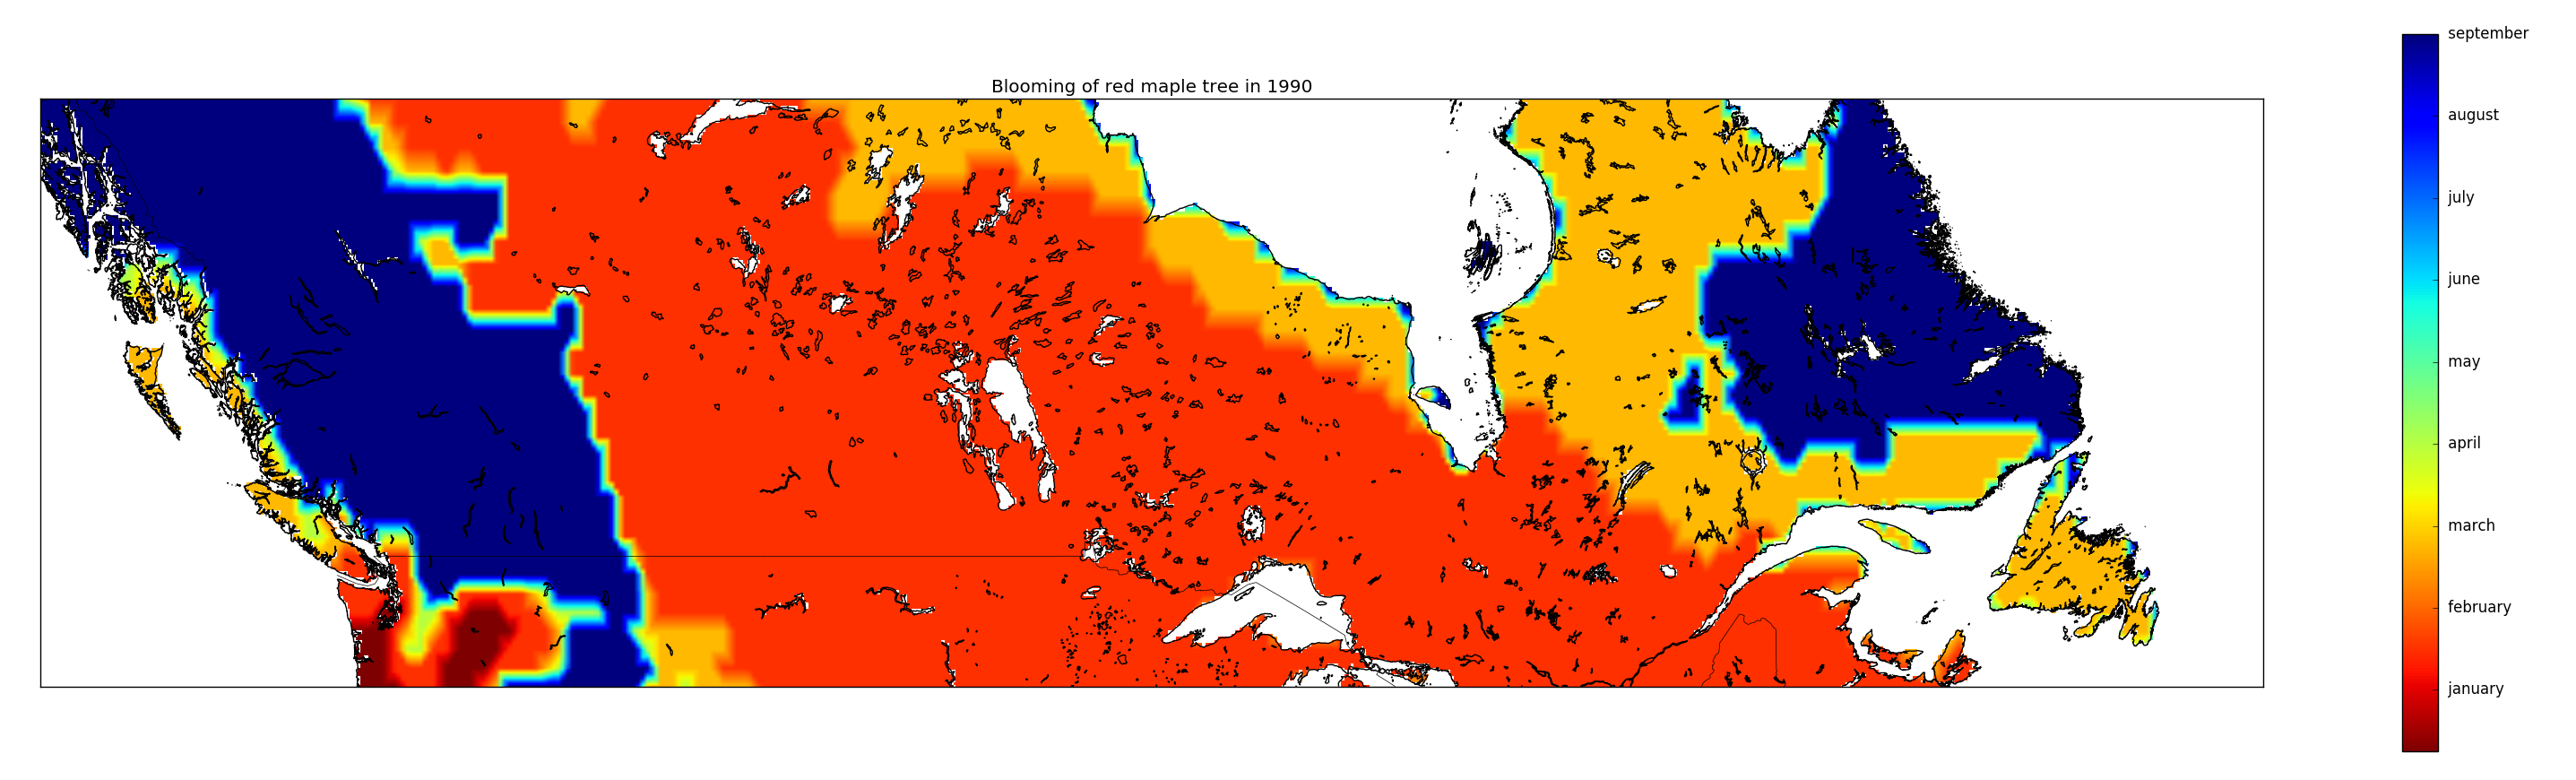
\includegraphics[width=0.9\textwidth]{./Output/CanadaBloomingOfMaple.png} 
		\caption{\scriptsize Figure shows the blooming month ovre Canada for the red maple tree.}\label{gddMapCaMaple}		  
	\end{figure}

\pagebreak
\begin{thebibliography}{2}
\bibitem[1]{gridTemp}\url{http://www.cccsn.ec.gc.ca/?page=dd-gcm}
\bibitem[2]{CityTemp}\url{http://climate.weather.gc.ca}
\end{thebibliography}


\end{document}
